
% Zeitz auskommentiert  \begin{center}                    
%   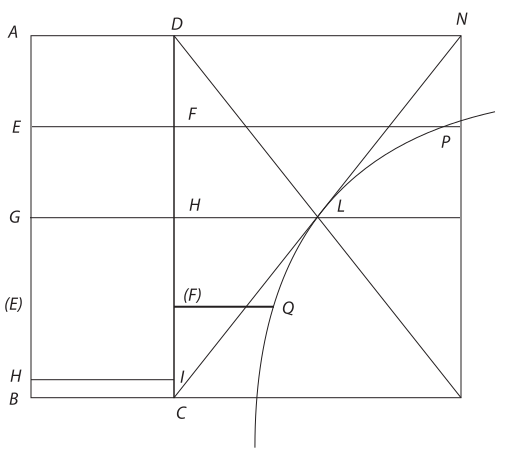
\includegraphics[width=0.45\textwidth]{images/35_5_5r1}\\\textit{[Fig. 5]}
%                        %\caption{Bildbeschreibung}
%   \end{center}
\pstart \footnotesize Quod si vero omnis aer \edtext{\textit{ABCD} seu \textit{bc}$\alpha$}{\lemma{}\Afootnote{\textit{ABCD} seu \textit{bc}$\alpha$ \textit{ erg.} \textit{ L}}} compressus sit in spatium $EBCF \sqcap b-y,\smallfrown c$ patet spatium in quod compressum est punctum aeris quodlibet (ob aequalem semper distributionem) esse ad spatium in quod compressum est quodlibet intruso omni aere in dimidium spatium rectanguli, esse ut \textit{EBCF}, ad \textit{GBCH}. Jam \edtext{vis}{\lemma{Jam}\Afootnote{ \textit{ (1) }\ punctum quodlibet aeris \textit{ (2) }\ eam \textit{ (3) }\ vis \textit{ L}}} quam exercet punctum quoddam aeris compressum est ad vim alterius minus magisve compressi in reciproca spatiorum \edtext{ratione. Ergo}{\lemma{ratione}\Afootnote{ \textit{ (1) }\ , seu si mavis in directa ratione materiae contentae; erit ergo \textit{ (2) }\ . Ergo \textit{ L}}} \textit{x}, vis aeris compressi\protect\index{Sachverzeichnis}{vis!aeris compressi} in spatium \textit{EBCF} \edtext{$\sqcap \hspace{4pt}b-y, \smallfrown c$}{\lemma{$\sqcap \hspace{4pt}b-y, \smallfrown c$}\Afootnote{ \textit{ erg.} \textit{ L}}} erit ad $\delta$ vim aeris compressi\protect\index{Sachverzeichnis}{vis!aeris compressi} in spatium $\displaystyle GBCH\sqcap\frac{bc}{2}$ ut $\displaystyle \frac{bc}{2}$ ad $b-y,\smallfrown c$, seu ut $\displaystyle \frac{b}{2}$ ad $b-y$. Ergo $\displaystyle x \sqcap\frac{\delta b}{2,\smallfrown b-y}$. Unde vis aeris\protect\index{Sachverzeichnis}{vis!aeris compressi} in spatium infinite parvum\protect\index{Sachverzeichnis}{spatium!infinite parvum} \textit{HBCI} compressi est infinita. Fiet enim $\displaystyle x \sqcap \frac{\delta b}{2,\smallfrown 0}$.\edlabel{sqcapstart}\edtext{}{\lemma{$\displaystyle x \sqcap \frac{\delta b}{2,\smallfrown 0}$.}\xxref{sqcapstart}{sqcapend}\Afootnote{ \textit{ (1) }\ Hinc jam manifeste patet  \textit{(a)}\ vires \textit{(b)}\ virium \textit{(c)}\ vires Elaterii\protect\index{Sachverzeichnis}{elaterium|textit} cylindrici compressi esse ut  \textit{(aa)}\ spatia \textit{(bb)}\ applicatas Hyperbolae \textit{CQLP} altitudine respondentes cujus Hyperbolae centrum \textit{D} in summo cylindrici: asymptotos ipsa cylindrici altitudo; vertex \textit{L} in recta \textit{GH} producta, mediam cylindrici altitudinem secante: latera rectum transversumque aequalia. Potentia seu rectangulum constans $\displaystyle \frac{\delta b}{2}$. \textit{ (2) }\ Hinc \textit{ L}}}
\pend
%Zeitz auskommentiert   \begin{center}
%   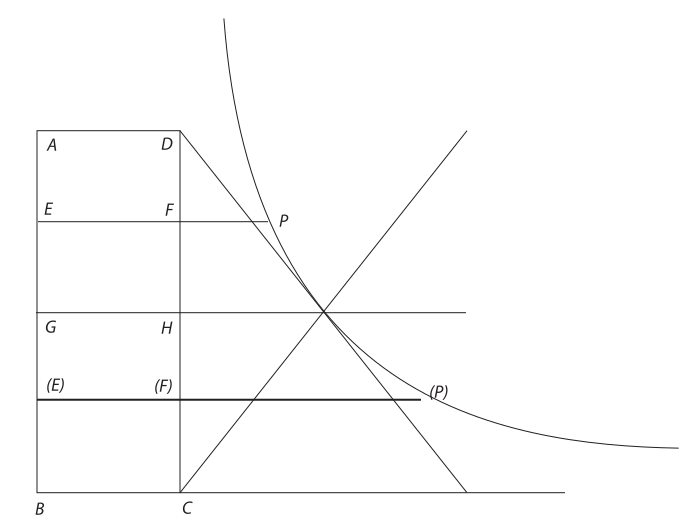
\includegraphics[width=0.64\textwidth]{images/35_5_5r2}\\\textit{[Fig. 6]}
%   \end{center}
\pstart \footnotesize Hinc\footnote{\textit{Links neben [Fig. 6]}: Rectius ita formabimus ut vertex Hyperbolae summo puncto \textit{D} respondeat.}  jam manifeste patet \edtext{\edlabel{sqcapend}progressionem}{\lemma{patet}\Afootnote{ \textit{ (1) }\ Hyperbolam \textit{ (2) }\ progressionem \textit{ L}}} virium Elaterii\protect\index{Sachverzeichnis}{vis!elaterii} cylindrici seu simplicis compressi esse ut applicatas ad Hyperbolae latus rectum transversumque aequale habentis, ad asymptoton. Posito \edtext{altitudines percursas}{\lemma{Posito}\Afootnote{ \textit{ (1) }\ centrum Hyperbolae esse in cylindrici Basi \textit{ (2) }\ spatia percursa\protect\index{Sachverzeichnis}{spatium!percursum|textit} esse abscissa \textit{ (3) }\ altitudines percursas \textit{ L}}} \edtext{\textit{DF} vel \textit{D(F)}}{\lemma{}\Afootnote{\textit{DF} vel \textit{D(F)} \textit{ erg.} \textit{ L}}} esse abscissas ex puncto in asymptoto sumto \edtext{\textit{D}}{\lemma{}\Afootnote{\textit{D} \textit{ erg.} \textit{ L}}}, versus centrum \textit{C}, in cylindrici basi, \edtext{distantiam}{\lemma{basi,}\Afootnote{ \textit{ (1) }\ rectangulum \textit{ (2) }\ distantiam \textit{ L}}} puncti sumti \edtext{\textit{D}}{\lemma{}\Afootnote{\textit{D} \textit{ erg.} \textit{ L}}}, a centro \textit{C}, esse \textit{b}. Potentiam hyperbolae esse $\displaystyle \frac{\delta b}{2}$. Unde caetera, latus scilicet rectum transversumque hoc loco aequalia, et quaevis ejus puncta \textit{P}, \textit{(P)} habentur; nempe patet ex figura adjecta, si \textit{DF}\edtext{}{\lemma{\textit{DF}}\Afootnote{\textbar\ sint \textit{ streicht Hrsg.}\ \textbar\ vel \textit{ L}\hspace{10cm}}} vel \textit{AE}, sint $\sqcap$ \textit{y} \textit{FP} fore \textit{x} ubicunque sumantur puncta, \textit{E}, \textit{F}, \textit{P}.\pend 
\pstart \footnotesize Etsi vero memorabile sit inprimis hoc theorema non tamen videtur esse ex difficillimis, ideoque crediderim etiam aliis animadversum.\footnote{\textit{Unter der Streichung}: Imo est error, ut patet pag. sequenti.}
\pend 
%Zeitz auskommentiert   \begin{center}                    
%   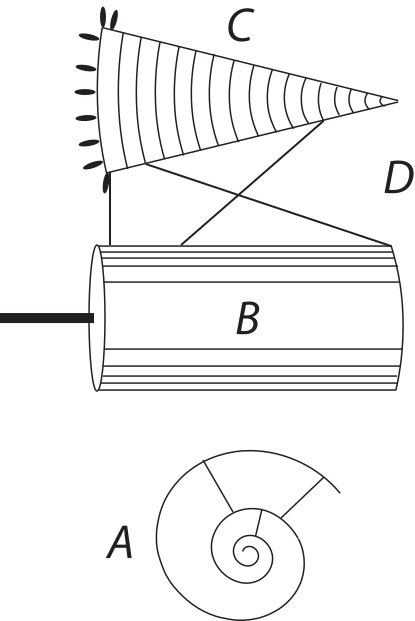
\includegraphics[width=0.27\textwidth]{images/35_5_5r3}\\\textit{[Fig. 7]}
%   \end{center}
   \clearpage
\pstart  \edtext{\edlabel{postuletstart}\textit{A} Elaterium\protect\index{Sachverzeichnis}{elaterium} \textit{B}}
{\lemma{\textit{A} Elaterium}\xxref{postuletstart}{postuletend}\Afootnote{[...] chordam \textit{D}  \textit{ (1) }\ fusum\protect\index{Sachverzeichnis}{fusum|textit} ad se \textit{ (2) }\ quam [...] majores  \textit{ (a) }\ spirae \textit{ (b) }\ circuli [...] nunc \textit{ (aa) }\ magis \textit{ (bb) }\ in se [...] ponemus \textit{ (aaa) }\ motum \textit{ (bbb) }\ effectum [...] si \textit{ (aaaa) }\ tubula \textit{ (bbbb) }\ tubuli sibi continue inditi essent. Qui  \textit{ (aaaaa) }\ in caeteros propagant flexum \textit{ (bbbbb) }\ flexu sibi [...] fingerentur, \textit{ (aaaaa-a) }\ de quo \textit{ (bbbbb-b) }\ quod hic [...] postulet. \textit{gestr. und wieder g\"ultig gemacht} \textit{ L}}} capsula Elaterii\protect\index{Sachverzeichnis}{elaterium}, \textit{C} fusum\protect\index{Sachverzeichnis}{fusum}. Elaterium\protect\index{Sachverzeichnis}{elaterium} se restituens circumagit capsulam \textit{B} quae per chordam \textit{D} quam ad se trahit fusum movet. Primum autem exiguis fusi spiris respondet, ita enim plurimum itineris facit motu, et plus effectus habet in horologio\protect\index{Sachverzeichnis}{horologium}, qui plus etiam Elaterio\protect\index{Sachverzeichnis}{elaterium} resistit. Quod ad compensationem pertinet, cum et fortius initio sit Elaterium\protect\index{Sachverzeichnis}{elaterium}, at ubi debilius nonnihil Elaterium\protect\index{Sachverzeichnis}{elaterium}, etiam majores circuli aguntur.
\pend
%Zeitz auskommentiert   \begin{center}
%   \includegraphics[width=0.3\textwidth]{images/35_5_5r4}
%   \includegraphics[width=0.3\textwidth]{images/35_5_5r5}\\\textit{[Fig. 8]}\hspace{3cm}\textit{[Fig. 9]}
%   \end{center}
\pstart Sed quicquid fit video spiram illam Elasticam parum aptam motui regendo. Nam ob spirae ipsius inaequalitatem variam consistentiam, et plicabilitatem fit, ut varie inter tendendum se formet, nunc in se ipsam recedendo, nunc sese instar arcus flectendo, nunc spiris invicem appropinquando. Quorum ut dixi certas regulas praescribere vix possibile est. Ut naturam arcus\protect\index{Sachverzeichnis}{arcus} et si licet figuram flexus exacte explicemus; quod utique sic satis difficile futurum est; ponemus effectum compositum ex motu et retentione: addemus flexibilitatem, velut si tubuli sibi continue inditi essent. Qui flexu sibi nonnihil educuntur. Quae eductio in omnes propagata foret, etamsi recta linea sibi educi aliqui tubi fingerentur, quod hic locum non habent. Sed ista inquisitio tam est subtilis tamque profunda, ut peculiarem sibi inquisitionem \edlabel{postuletend}postulet.%
\footnote{\textit{Quer zum wieder g\"{u}ltig gemachten Text}: NB Quae inclusa hic deleri non debent. NB \textit{dreimal unterstrichen.}}
\pend 
%Zeitz auskommentiert   \begin{center}
%   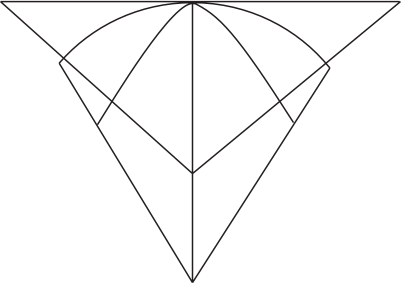
\includegraphics[width=0.2\textwidth]{images/35_5_5r6}
%   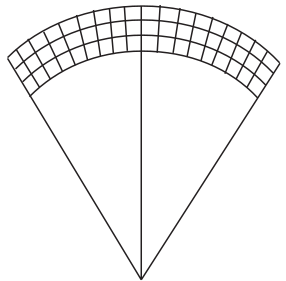
\includegraphics[width=0.2\textwidth]{images/35_5_5r7}
%   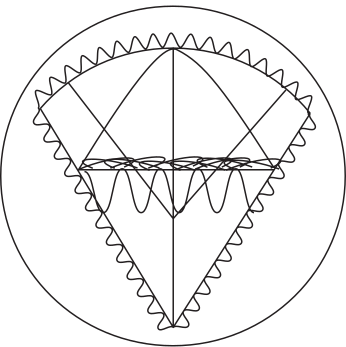
\includegraphics[width=0.2\textwidth]{images/35_5_5r8}
%   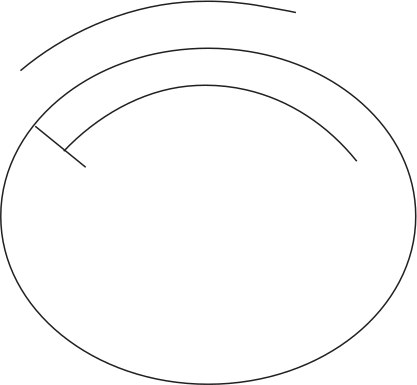
\includegraphics[width=0.2\textwidth]{images/35_5_5r9}\\\hspace{0.2cm}\textit{[Fig. 10]}\hspace{1.2cm}\textit{[Fig. 11]}\hspace{1.3cm}\textit{[Fig. 12]}\hspace{1.3cm}\textit{[Fig. 13]}
%   \end{center}
\pstart \footnotesize Quod dixisse visus sum; esse \edtext{vim}{\lemma{esse}\Afootnote{ \textit{ (1) }\ Elateri \textit{ (2) }\ vim \textit{ L}}} compressorum in reciproca spatiorum ratione, quae implent falsum est. Nam aeris in spatio \textit{ADBC} vis est = 0.\footnote{\textit{Interlinear \"{u}ber der} 0: Error.} seu infinite parva in spatio\protect\index{Sachverzeichnis}{spatium!infinite parvum} \textit{GBCH} est finita satis magna; cum tamen spatia sint in dupla ratione. Alia ergo determinatio quaerenda est, nihilque hactenus actum.\pend 
\pstart  \footnotesize Nimirum vis omnis quam exercet aer compressus ad se restituendum oritur a difformitate ejus a circumjacente. Cum sit circumjacens aer, qui eum retineat seu qui vim ejus compenset, cum est in statu naturali\protect\index{Sachverzeichnis}{status naturalis}. Absolute loquendo, sive in vacuo si nullum ponamus esse densitatis statum\protect\index{Sachverzeichnis}{status naturalis} aeri naturalem, sed vim Elaterii\protect\index{Sachverzeichnis}{vis!elaterii} esse ad expandendum sese in infinitum, verum id erit spatiumque inter duas Asymptotos Hyperbolae curvamque comprehensum perfecte vim illam repraesentabit. Sed ista ad usum non pertinent, \edtext{quo}{\lemma{pertinent,}\Afootnote{ \textit{ (1) }\ ubi \textit{ (2) }\ quo \textit{ L}}} censetur aliquis esse status\protect\index{Sachverzeichnis}{status naturalis} aeri naturalis, ubi vis Elaterii\protect\index{Sachverzeichnis}{vis!elaterii} nulla. Cum ergo vires sint majores quo major est diversitas aeris circumjecti, et aeris compressi; quaeritur an aestimanda vis sit ex differentiis an ex rationibus aeris compressi et circumjecti. Ante omnia manifestum est, vim aeris in \textit{ABCD} esse nullam, quia aequali vi sese expandendi aeris compressi compensatur in \textit{EBCF} vis aeris \edtext{ad}{\lemma{aeris}\Afootnote{ \textit{ (1) }\ est \textit{ (2) }\ ad \textit{ L}}} circumjectum, ut aucta est ob auctam difformitatem, id est ob auctam rationem materiae ad spatium, id est ob spatium manente quippe materia diminutione. Itaque \edtext{vis}{\lemma{Itaque}\Afootnote{ \textit{ (1) }\ aer \textit{ (2) }\ vis \textit{ L}}} augebitur spatii diminutionibus; et \edtext{spatio reddito}{\lemma{et}\Afootnote{ \textit{ (1) }\ vi re \textit{ (2) }\ spatio reddito \textit{ L}}} infinite parvo vis erit infinita, spatio reddito \textit{ABCD} vis erit nulla. (Imo haec objectio est erronea ut patet ex pag. sequenti. Interim tamen et ratiocinatio procedens fuit etiam erronea, ut ex eadem patebit.)\pend